\documentclass[12pt]{kiarticle} % You can learn about my document class "kiarticle" and install it to your device by following the link: https://github.com/Kiarendil/toolkitex
\graphicspath{{pictures/}}
\DeclareGraphicsExtensions{.pdf,.png,.jpg,.eps}
%%%
\pagestyle{fancy}
\fancyhf{}
%\renewcommand{\headrulewidth}{ 0.1mm }
\renewcommand{\footrulewidth}{ .0em }
\fancyfoot[C]{\texttt{\textemdash~\thepage~\textemdash}}
\fancyhead[L]{Лабораторная работа № 3.3.2 \hfil}
\fancyhead[R]{\hfil Иванов Кирилл, 625 группа }
\usepackage{multirow} % Слияние строк в таблице
\newcommand
{\un}[1]
{\ensuremath{\text{#1}}}



\begin{document}

\begin{titlepage}
	\begin{center}
		\large 	Московский физико-технический университет \\
		Факультет общей и прикладной физики \\
		\vspace{0.2cm}
		
		\vspace{4.5cm}
		Лабораторная работа № 3.3.2 \\ \vspace{0.2cm}
		\large (Общая физика: электричество и магнетизм) \\ \vspace{0.2cm}
		\LARGE \textbf{Исследование вольт-амперной характеристики вакуумного диода, или "<Закон трех вторых">}
	\end{center}
	\vspace{2.3cm} \large
	
	\begin{center}
		Работу выполнил: \\
		Иванов Кирилл,
		625 группа
		\vspace{10mm}
		
	
		
		
	\end{center}
	
	\begin{center} \vspace{60mm}
		г. Долгопрудный \\
		 2017 год
	\end{center}
\end{titlepage}




\paragraph*{Цель работы:} определение удельного заряда электрона на основе "<закона трех вторых">.

\paragraph*{Оборудование:} радиолампа с цилиндрическим анодом, амперметр, многопредельные микроамперметр и вольтметр постоянного тока, стабилизированные источники постоянного тока и постоянного напряжения.


\section{Историческая справка}

\textbf{Закон степени трёх вторых} (закон Чайлда, закон Чайлда-Ленгмюра, закон Чайлда-Ленгмюра-Богуславского) ---  в электровакуумной технике задаёт квазистатическую вольт-амперную характеристику идеального вакуумного диода --- зависимость тока анода от напряжения между его катодом и анодом --- в режиме пространственного заряда.

\begin{equation}\label{}
I \sim V^{3/2}
\end{equation}

Первую формулировку закона предложил в 1911 году Чайлд (англ.), впоследствии закон был уточнён и обобщён работавшими независимо друг от друга Ленгмюром (1913), Шоттки (1915) и Богуславским (1923). Закон, c оговорками, применяется и к лампам с управляющей сеткой (триоды, тетроды) и к электронно-лучевым приборам. Закон применим для области средних напряжений — от нескольких В до напряжений, при которых начинается переход в режим насыщения тока эмиссии. Закон не применим к области отрицательных и малых положительных напряжений, к области перехода в режим насыщения и к самому режиму насыщения.

\section{Теоретическое введение}
\begin{wrapfigure}{l}{0.35\linewidth} 
	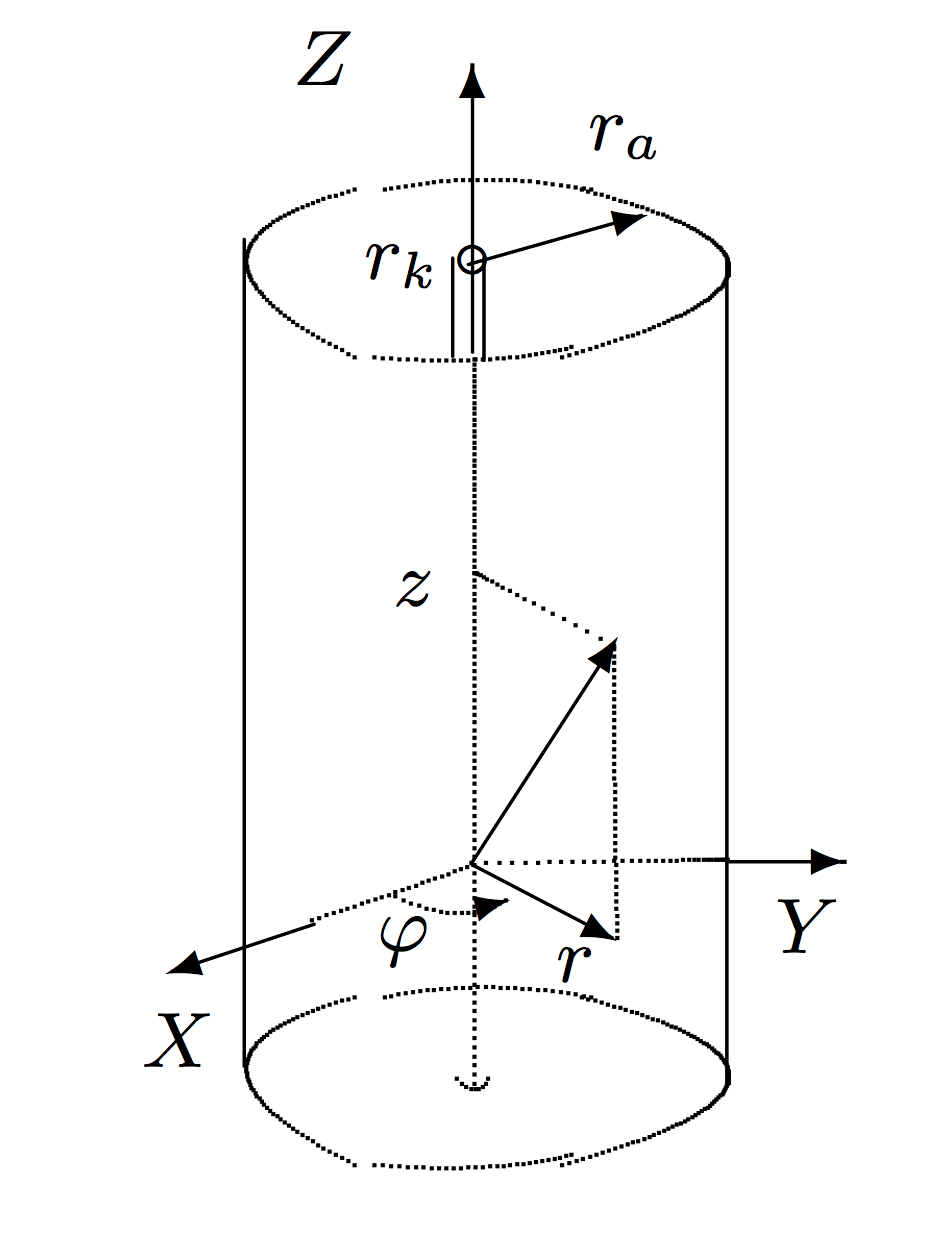
\includegraphics[width=6cm]{diod}
	\caption{Схема распределения электродов в диоде}
\end{wrapfigure}

В работе исследуется зависимости прямого тока, проходящего через вакуумный диод, в зависимости от напряжения на нем, а именно та часть вольт-амперной характеристики, в которой электронное облако существенно влияет на распределение электрического поля между катодом и анодом.

Распределение потенциала по радиусу внутри диода определяется уравнением Пуассона в цилиндрических координатах:

\begin{equation}\label{}
\Delta V = \dfrac{d^2V}{dr^2} + \dfrac{1}{r} + \dfrac{dV}{dr} = - \dfrac{\rho(r)}{\epsilon_0}
\end{equation}

При этом плотность заряда $ \rho(r) $ связана с текущим через слой диода толщины $ l $ током $ I $ формулой $ I = -2\pi r \rho(r)v(r)l$. При этом из закона сохранения энергии мы легко находим скорость $ v(r) $ электронов , прошедших через разность потенциалов $ V(r) $: $ \frac{mv^2}{2} = eV(r) $.  Отсюда мы получаем уравнение 

\begin{equation}\label{ur}
r \dfrac{d^2V}{dr^2} + \dfrac{dV}{dr} = \dfrac{I}{2\pi\epsilon_0}\sqrt{\dfrac{m}{2eV}}
\end{equation}

Однако, в дифференциальном уравнении 2-ого порядка относительно $ V(r) $ нам неизвестен ток I, зависящий от V. Для доопределения уравнения будем полагать:

\begin{equation}\label{usl}
\dfrac{dV}{dt}\bigg |_{r=r_k} = 0
\end{equation} 

Наше предположение означает что вблизи катода пространственный заряд электронов полностью экранирует поле анодной разности потенциалов.

Уравнение \eqref{ur} является нелинейным. Попробуем  найти некое частное решение, где $ V_a = V_{a0}, $ при котором ток $ I = I_0 $. Тогда выражения 

\begin{equation}\label{}
I = I_o \left( \dfrac{V_a}{V{a0}} \right) ^{3/2}, \qquad V(r) = V_{a0}(r)\dfrac{V_a}{V_{a0}}
\end{equation}

являются решением уравнения \eqref{ur}, что проверяется подстановкой. В общем виде решение записывается в виде

\begin{equation}\label{3/2}
I = \dfrac{8\sqrt{2}\pi \epsilon_0 l}{9}\sqrt{\dfrac{e}{m}}\dfrac{1}{r_a\beta^2} V^{3/2}
\end{equation}

Это и есть так называемый "<закон трех вторых"> -- ток в вакуумном диоде пропорционален напряжению на нем в степени 3/2. Он справедлив при любой геометрии электродов, если ток не слишком велик (т.е. пока выполнено условие \eqref{usl}). 

Так как нам нужно найти удельный заряд электрона, выпишем в явном виде его из уравнения \eqref{3/2}:

\begin{equation}\label{e/m}
\dfrac{e}{m} = \dfrac{81r_a^2\beta^4}{128\pi^2\epsilon_0^2l^2} \x \dfrac{I^2}{V^2} = k \x \dfrac{I^2}{V^2}
\end{equation}

Таким образом, удельный заряд электрона определяется из отношения квадрата тока к кубу напряжения, умноженный на коэффициент, зависящий от параметров установки.

\section{Экспериментальная установка}
\begin{figure}[h]
	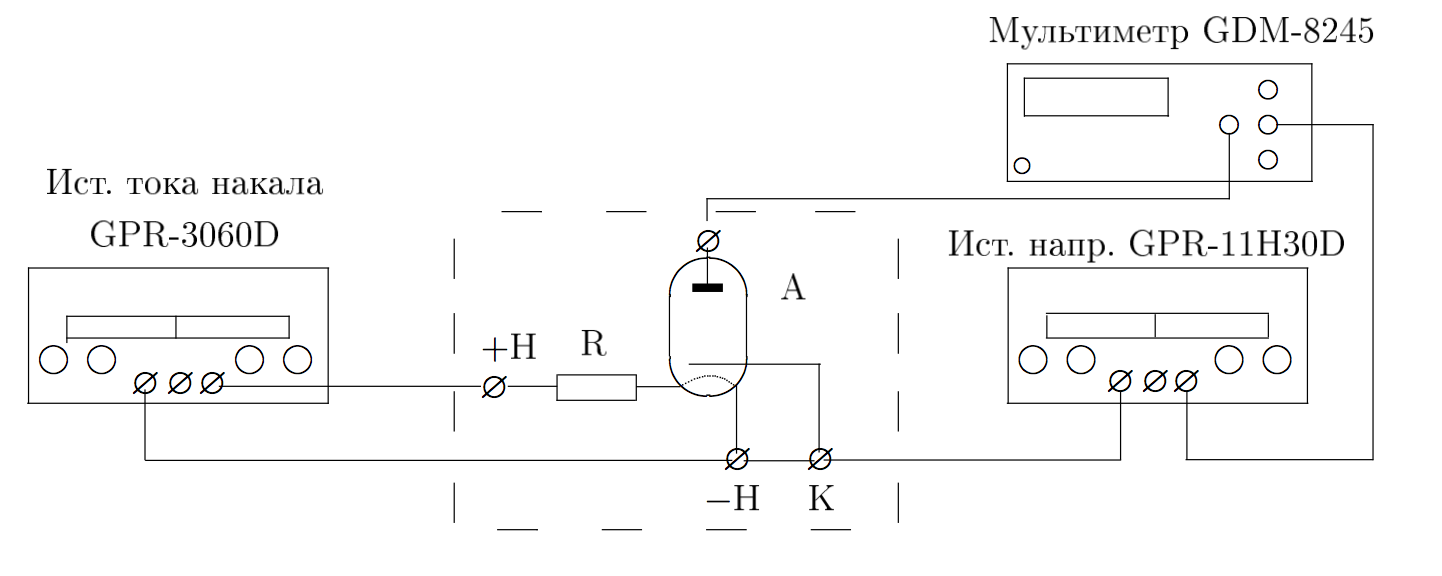
\includegraphics[width=15cm]{lab}
	\caption{Схема экспериментальной установки}
\end{figure}

В работе используется диод 2Ц2С с косвенным накалом. Радиус его катода $ r_k = 0,9 $ мм, радиус анода $ r_a = 9,5  $ мм, коэффициент $ \beta^2 = 0,98 $, длина слоя центральной части катода, покрытой оксидным слоем $ l = 9 $ мм.

Для подогрева катода и анода используются стабилизированные источники постоянного тока и напряжения. В цепь накала включено предохранительное напряжение $ R $. Анодное напряжение измеряется вольтметром источника питания, анодный ток --- многопредельным мультиметром GDM-8245. 


\section{Ход работы}

Вычислим коэфициент $ k $:

\begin{equation}\label{}
k = \dfrac{81r_a^2\beta^4}{128\pi^2\epsilon_0^2l^2} = \dfrac {81\x(9,5\x10^{-3})^2\x0,98^4}{64\x2\x3,14^2\x(8,85\x10^{-12})^2\x(9\x10^{-3})^2} \backsimeq 8,4 \x 10^{20}
\end{equation}

Установим ток накала на $ I_н = 1,3 $ А, а начальное анодное напряжение на $ V = 0.5  $ В.  Проведем измерения анодного тока в зависимости от напряжения, изменяя его от $ 0,5 $ до 50 В. 

Затем проведем аналогичные измерения для других токов накала: $ 1,4, 1,5, 1,6 $ А. Результаты занесем в таблицу \ref{res}.

\begin{table}
	\centering
	\caption{Результаты измерений}
\begin{tabular}{|c|c|c|c|c|c|c|c|c|}
	\hline
	\multirow{2}{*}{$ V $, В}& \multicolumn{2}{|c|}{$ I_н = 1,3  $А}  & \multicolumn{2}{|c|}{$ I_н = 1,4  $А} & \multicolumn{2}{|c|}{$ I_н = 1,5  $А} & \multicolumn{2}{|c|}{$ I_н = 1,6  $А} \\
 \cline{2-9}
 & \text{I, мкА} &$ \frac{I^2}{V^3}, \frac{\un{мкА}^2}{\un{В}^3}$ & \text{I, мкА} & $ \frac{I^2}{V^3}, \frac{\un{мкА}^2}{\un{В}^3}$ &\text{I, мкА}
& $ \frac{I^2}{V^3}, \frac{\un{мкА}^2}{\un{В}^3}$  &\text{I, мкА}& $ \frac{I^2}{V^3}, \frac{\un{мкА}^2}{\un{В}^3}$  \\
\hline
 0.5 & 3.64 & 105.997 & 5.56 & 247.309 & 11.86 & 1125.28 & 18.82 & 2833.54 \\
 1 & 11.93 & 142.325 & 13.31 & 177.156 & 21.68 & 470.022 & 31.83 & 1013.15 \\
 1.5 & 21.75 & 140.167 & 25.62 & 194.484 & 37.08 & 407.386 & 38.07 & 429.43 \\
 2 & 34.51 & 148.868 & 41.41 & 214.349 & 52.69 & 347.03 & 64.02 & 512.32 \\
 2.5 & 48.17 & 148.502 & 57.05 & 208.301 & 70.39 & 317.104 & 85.53 & 468.184 \\
 3 & 63.75 & 150.521 & 74.19 & 203.858 & 88.15 & 287.793 & 104.7 & 406.003 \\
 3.5 & 81.05 & 153.215 & 92.66 & 200.254 & 108.2 & 273.055 & 126.1 & 370.874 \\
 4 & 100.3 & 157.189 & 114.5 & 204.848 & 130.7 & 266.914 & 151.9 & 360.525 \\
 4.5 & 123 & 166.025 & 136.6 & 204.769 & 151.6 & 252.209 & 172.6 & 326.922 \\
 5 & 141.3 & 159.726 & 157.7 & 198.954 & 175.5 & 246.402 & 197.9 & 313.315 \\
 5.5 & 163.7 & 161.068 & 181.3 & 197.564 & 200.2 & 240.902 & 223.8 & 301.045 \\
 6 & 188.8 & 165.025 & 206.1 & 196.654 & 228.7 & 242.147 & 253.75 & 298.098 \\
 7 & 239.3 & 166.952 & 259.9 & 196.933 & 384.93 & 431.986 & 319.3 & 297.238 \\
 8 & 297.1 & 172.399 & 319.9 & 199.875 & 346.15 & 234.023 & 377.7 & 278.628 \\
 9 & 356.2 & 174.044 & 380.5 & 198.601 & 405.9 & 226.001 & 441.1 & 266.899 \\
 10 & 419.4 & 175.896 & 446.53 & 199.389 & 505.9 & 255.935 & 553.1 & 305.92 \\
 15 & 815.9 & 197.242 & 856.2 & 217.208 & 903.1 & 241.656 & 954.1 & 269.721 \\
 20 & 1297 & 210.276 & 1343 & 225.456 & 1394 & 242.905 & 1460 & 266.45 \\
 25 & 1834 & 215.268 & 1899 & 230.797 & 1993 & 254.211 & 2043 & 267.126 \\
 30 & 2436 & 219.781 & 2522 & 235.573 & 2596 & 249.601 & 2680 & 266.015 \\
 35 & 3076 & 220.683 & 3184 & 236.451 & 3273 & 249.855 & 3363 & 263.785 \\
 40 & 3796 & 225.15 & 3905 & 238.266 & 3994 & 249.251 & 4108 & 263.682 \\
 45 & 4488 & 221.039 & 4666 & 238.92 & 4770 & 249.689 & 4889 & 262.303 \\
 50 & 5333 & 227.527 & 5554 & 246.775 & 5676 & 257.736 & 5797 & 268.842 \\
	\hline

\end{tabular}% 
\label{res}% 
\end{table}% 

Из теории известно, что "<закон трех вторых"> верен только на некотором участке вольт-амперной характеристики. Из формулы \eqref{e/m} и физического смысла понятно, что отношение $ \frac{I^2}{V^3} $ должно быть постоянным (ведь оно пропорционально фундаментальной константе). Из таблицы \ref{res} видно, что для каждого тока напряжения можно выделить искомое отношение, которое остается постоянным на большом числе точек и только на нем. Применим для него распределение Стьюдента с 95\% доверительным интервалом (двусторонним). При этом погрешность выбора нашего отношения (обозначим его за $ a $) будем считать по формуле

\begin{equation}\label{sigma}
a = \bar{a} \pm \sigma_a, \qquad \sigma_a = A \x \dfrac{S(a)}{\sqrt{N}}
\end{equation} 

Где $ A $ --- коэффициент Стьюдента, $ S(a) $ --- среднеквадратичное отклонение. Результаты запишем в таблицу \ref{st}.

\begin{table}
	\centering
	\caption{Обработка результатов}
\begin{tabular}{|c|c|c|c|c|c|c|}
	\hline
	$ I_н $, А & $ a, \frac{\un{мкА}^2}{\un{В}^3} $ & $ N $ & $ S(a), \frac{\un{мкА}^2}{\un{В}^3} $ & $ A $ & $ \sigma_{\bar{a}}, \frac{\un{мкА}^2}{\un{В}^3} $ & $ \bar{a}, \frac{\un{мкА}^2}{\un{В}^3} $ \\
	\hline
	1.3 & 160 & 7 & 5 & 2.447 & 4.7 & 161.3 \\
	1.4 & 200 & 13 & 4 & 2.179 & 3.3 & 200.3 \\
	1.5 & 240 & 15 & 7 & 2.145 & 5.7 & 246.9 \\
	1.6 & 265 & 9 & 2.5 & 2.306 & 2.1 & 266.1 \\
	\hline
\end{tabular}
\label{st}% 
\end{table}% 

Теперь вычислим искомое значение удельного заряда электрона по формуле \eqref{e/m} для получившихся значений $ \frac{I^2}{V^3} $ (подставляя вместо нашего соотношения $ \bar{a} $):

\begin{equation}\label{}
\dfrac{e}{m} = k \x \bar{a} \pm \sigma_{\frac{e}{m}}, \qquad \sigma_{\frac{e}{m}} = \frac{e}{m} \x \dfrac{\sigma_{\bar{a}}}{\bar{a}}
\end{equation}

Для тока накала $ I_н = 1,3 $ А мы получаем $ \dfrac{e}{m} = (1,359 \pm 0,039) \x 10^{11} \dfrac{\un{Кл}}{\un{кг}}$. 

Для тока накала $ I_н = 1,4 $ А мы получаем $ \dfrac{e}{m} = (1,757 \pm 0,029)  \x 10^{11} \dfrac{\un{Кл}}{\un{кг}}$. 

Для тока накала $ I_н = 1,5 $ А мы получаем $ \dfrac{e}{m} = (2,079 \pm 0,048)  \x 10^{11} \dfrac{\un{Кл}}{\un{кг}}$. 

Для тока накала $ I_н = 1,6 $ А мы получаем $ \dfrac{e}{m} = (2,241 \pm 0,018)  \x 10^{11} \dfrac{\un{Кл}}{\un{кг}}$. 


\section{Вывод}

Табличное значение удельного заряда электрона равно $ 1, 759  \x 10^{11} \dfrac{\un{Кл}}{\un{кг}} $. Под него подходит только результат, полученный при токе накала $ I_н = 1,4 $ А:


\begin{center}
{\fbox{ $ \dfrac{e}{m} = (1,757 \pm 0,029)  \x 10^{11} \dfrac{\un{Кл}}{\un{кг}}$}} \\
\end{center} 

Как мы видим, данный метод позволяет определить удельный заряд электрона с точностью до порядка величины ($ \simeq  10^{11} \dfrac{\un{Кл}}{\un{кг}} $). Однако с табличным значением совпадает только один из четырех результатов.


\end{document}